

%\addcontentsline{toc}{chapter}{Development Process}
\chapter{Design}
\label{Design}

This section will describe the design of the project.
While the background chapter describes the overall problems and aims of the project, this chapter describes the overall design of the project and creates an outline in which the project is implemented.

\section{Environment Design}
The final environment for this project will consist of one large room with obstacles placed in it. \\
The program will be tested on a number of different sized rooms with different amount and sized obstacles in it.

\begin{figure}[h]
\centering
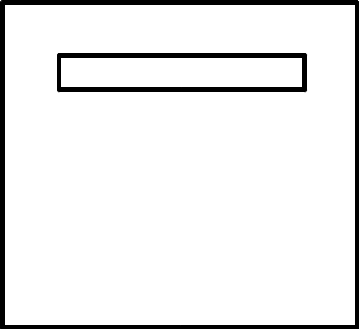
\includegraphics[width=0.5\textwidth]{../../figures/environment_example2.png} 
\caption{Environment Design}
\label{Figure 2}
\end{figure}

\section{Mapping}
For mapping a occupancy grid will be used, and the occupancy will be acquired by the E-Puck's distance sensors. 
One robot will be used to move around and map the environment. 

\section{Deployment}
In this section the considered deployment algorithms are described, as well as the reasons as to why the one which has been implemented was chosen rather than the other. 

\subsection{Considered Deployment algorithms}
\subsubsection{Strategy 1}
One which is based on a random walk though the environment which will turn to a random heading when an obstacle has been reached. \\
This approach could be combined with a wall following algorithm which would trigger a random walk when the same position is reached again. This would allow for the complete traverse of a obstacle/wall. This would require a good localisation solution as without it the robot will be stuck inside an eternal loop.\\
\subsubsection{Strategy 2}
The other deployment strategy would implement a more controlled movement pattern. This pattern would move the robots inside a rectangular pattern which would implement a function to move around obstacles on the way before moving back into the original pattern. \\[3ex]

While at this point it is unsure which approach(or combination of approaches) would be more effective, out of time limitation only one algorithm will be implemented. Other approaches might be considered in future implementations. 

\begin{figure}[h]
\centering
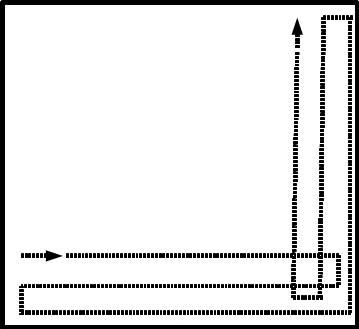
\includegraphics[width=0.5\textwidth]{../../figures/movement_pattern.png} 
\caption{Controlled movement Pattern}
\label{Figure 3}
\end{figure}

\subsection{Adopted design}
It was decided to adopt and implement \textbf{strategy 2} which can be seen in figure \ref{Figure 3}.\\
The reason for this being that the developer believes a random walking approach, because of its random behaviour, would be more problematic in a more complex environment whereas the controlled movement pattern(strategy 2) would perform better.\\
The reason that \textbf{strategy 1}, the random walking approach, is considered to perform in worse in a more complex environment is because of the nature of odometry calculations and the environment. In the earliest implementation iterations the non-accurate nature of odometry was discovered. \\
Odometry calculations are more an estimate of the robots absolute position rather than an accurate calculation. The reason odometry is not 100\% accurate is because sensor noise in the E-Pucks stepper motor encoders and the simulated friction between the wheels and the floor. \\[3ex]

This leads to inaccuracy while turning and moving. A random movement approach would make the already inaccurate calculations even more inaccurate as in a more controlled approach with a static movement pattern turn angles and directions of movement can be pre set and algorithms designed to control these. \\
In addition to these reasons, mapping in straight line patterns allow for more accurate mapping of walls and force the robot to cover the whole environment.\\
Of course strategy 2 is not without it downsides as will be shown in the chapter 4, on page \pageref{Testing}. However these downsides are considered less of a problem as the random walking approach.

\begin{figure}[h]
\centering
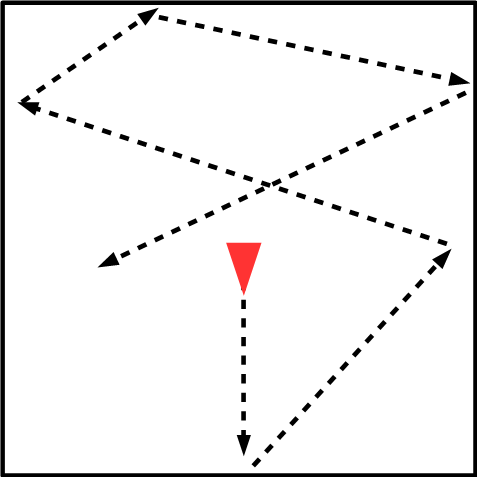
\includegraphics[width=0.5\textwidth]{../../figures/random_walking.png} 
\caption{The problem with the random walking approach}
\label{random_walking}
\end{figure}

Figure \ref{random_walking} display the downside with a random walking approach(strategy 1). \\
The \textit{red} arrow indicates the robot's start position. 
As the robot by definition will turn in a random angle it can not be guaranteed that the robot will cover the whole environment with its movement. Even if it would be \textit{assumed} that the robot would cover the entire environment its random behaviour would create problems for concise mapping. 
